\documentclass[11pt,a4paper]{article}

\usepackage[margin=2.4cm]{geometry}
\usepackage{amsmath,amssymb}
\usepackage{graphicx}
\usepackage{booktabs}
\usepackage[font=small,labelfont=bf]{caption}

\usepackage{xcolor}
\usepackage{listings}

\definecolor{codebg}{HTML}{F7F7F7}
\definecolor{codecomment}{HTML}{6A737D}
\definecolor{codekeyword}{HTML}{005CC5}
\definecolor{codestring}{HTML}{032F62}

\lstdefinestyle{python}{
  language=Python,
  backgroundcolor=\color{codebg},
  basicstyle=\ttfamily\footnotesize,
  keywordstyle=\color{codekeyword}\bfseries,
  commentstyle=\color{codecomment}\itshape,
  stringstyle=\color{codestring},
  numbers=left,
  numberstyle=\tiny\color{gray},
  numbersep=8pt,
  frame=single,
  rulecolor=\color{gray!40},
  breaklines=true,
  breakatwhitespace=false,
  postbreak=\mbox{\textcolor{gray}{$\hookrightarrow$}\space},
  showstringspaces=false,
  keepspaces=true,
  columns=fullflexible,
  tabsize=4,
  upquote=true,
  captionpos=b,
}

\usepackage[hidelinks]{hyperref}
\usepackage{tikz}
\usetikzlibrary{calc}
\usepackage{subcaption}
\usepackage{float}

\graphicspath{{figures/}}

\title{Topological \& Structural Analysis of the Indian Stock Market}
\author{ECS414 -- Network Science Theory and Applications}
\date{November 2026}


\begin{document}



% ---------------------------------------------------------------- title page
\begin{titlepage}
\begin{tikzpicture}[remember picture,overlay]
\draw[line width=0.5pt]
    ($(current page.north west)+(2.2cm,-2.2cm)$)
    rectangle
    ($(current page.south east)+(-2.2cm,2.2cm)$);
\end{tikzpicture}
\centering
\vspace*{3.5cm}
{\Large ECS414 -- Network Science Theory and Applications}\\[1.0cm]
{\Huge\bfseries Topological \& Structural Analysis\par}
{\Huge\bfseries of the Indian Stock Market}\\[2.1cm]
{\LARGE\bfseries Assignment}\\[2.5cm]
{\large by}\\[2.4cm]
{\large Divyam Sood}\\[0.4cm]
{\large Roll No: 23112}\\[4.4cm]
{\large 19 November 2026}
\vfill
\end{titlepage}

\tableofcontents
\newpage

% ---------------------------------------------------------------- introduction
\section{Introduction}
\label{sec:intro}
Financial markets are archetypal complex systems: thousands of interacting
assets generate collective behaviour that cannot be understood from individual
stocks alone. A useful abstraction is to treat stocks as nodes and strong
statistical dependencies between their returns as edges. The resulting
\emph{correlation network} makes concepts such as hubs, bridges, communities
and robustness directly measurable with network science.

The objective of this assignment is to construct, visualise, and analyse a complex network of stocks from the Indian National Stock Exchange (NSE) using historical price data. Students will investigate how market dynamics, sector
correlations, and structural hubs emerge from time-series data using foundational concepts in network
science.

\section{Methodology}
\label{sec:methods}

\subsection{Data source and preprocessing}
The constituent list \texttt{ind\_nifty200list.csv} supplies 200 symbols and
their NSE \texttt{Industry} labels. Daily prices for the period 20~November~2023 to
18~November~2026 (three years, 740 trading dates) were downloaded in one
\texttt{yfinance} request with \texttt{auto\_adjust=True}, so the
\texttt{Close} series is dividend/split-adjusted. All downloaded prices are cached in
\texttt{data/prices\_raw.csv}, so no later step repeats a network request as suggested in the assignment.

% Optional: raw yfinance download and local cache
% % ---------------------------------------------------------------------------
% Code snippet: adjusted-price download and local caching
% Source file: src/00_fetch_data.py
% Suggested placement: Section 2.1 (Data source and preprocessing).
% Uses the shared 'python' listings style defined in main.tex.
% ---------------------------------------------------------------------------
\begin{lstlisting}[style=python]
# Build NSE tickers from the constituent list
constituents = pd.read_csv(config.CONSTITUENTS_CSV)
tickers = [f"{symbol}.NS"
           for symbol in constituents["Symbol"].astype(str)]

# One batch request for all 200 symbols
data = yf.download(
    tickers,
    period=config.PERIOD,          # "3y"
    interval=config.INTERVAL,      # "1d"
    auto_adjust=True,              # 'Close' is the adjusted close
    progress=False,
    threads=True,
    group_by="column",
)

# Keep the close series and cache it, so later steps never hit the network
close = data["Close"] if isinstance(data.columns, pd.MultiIndex) else data
close = close.dropna(axis=1, how="all")
close.index.name = "Date"
close.to_csv(config.PRICES_RAW_CSV)
\end{lstlisting}


For stock $i$ on day $t$, the logarithmic return is
\begin{equation}
  r_{i,t}=\ln\!\left(\frac{P_{i,t}}{P_{i,t-1}}\right)
  \label{eq:returns}
\end{equation}
Stocks with price coverage below $80\%$ of the
trading dates were discarded. Seven dates were also dropped: 20--24 and
28~November~2023, and 15~January~2026. This yields 186 stocks and 732 daily
return observations.

% ---------------------------------------------------------------------------
% Code snippet: coverage filter, log returns and Pearson correlation
% Source file: src/01_preprocess.py
% Suggested placement: Section 2.1-2.2 (equations 1 and 2).
% Uses the shared 'python' listings style defined in main.tex.
% ---------------------------------------------------------------------------
\begin{lstlisting}[style=python]
# Drop stocks with less than 80% price coverage, then isolated-gap dates
coverage = prices.notna().mean()
dropped = sorted(
    [(ticker, float(coverage[ticker])) for ticker in prices.columns
     if coverage[ticker] < config.MIN_COVERAGE],
    key=lambda x: x[1],
)
prices = prices.drop(columns=[t for t, _ in dropped])
prices = prices.dropna(axis=0, how="any")

# Log returns, eq. (1)
returns = np.log(prices).diff().dropna(how="any")

# Pearson correlation matrix, eq. (2)
min_periods = int(config.MIN_COVERAGE * len(returns))
corr = returns.corr(method="pearson", min_periods=min_periods)

# Sanity checks: symmetric, unit diagonal, no missing pairs
assert np.allclose(corr.to_numpy(), corr.to_numpy().T, equal_nan=True)
assert np.allclose(np.diag(corr.to_numpy()), 1.0)
assert corr.notna().all().all()
\end{lstlisting}


\subsection{Correlation and network construction}
For every pair of stocks we compute the Pearson correlation of their return
series,
\begin{equation}
  \rho_{ij}=\frac{\sum_t (r_{i,t}-\bar r_i)(r_{j,t}-\bar r_j)}
                 {\sqrt{\sum_t (r_{i,t}-\bar r_i)^2}\,
                  \sqrt{\sum_t (r_{j,t}-\bar r_j)^2}}.
  \label{eq:pearson}
\end{equation}
The unweighted adjacency matrix is
\begin{equation}
  A_{ij}=\begin{cases}
    1 & \rho_{ij}\ge r,\; i\ne j,\\
    0 & \text{otherwise},
  \end{cases}
  \label{eq:adjacency}
\end{equation}
so an edge means ``these two stocks moved together more strongly than the
chosen threshold $r$''. The graph is simple and undirected, and the underlying
$\rho_{ij}$ is retained as an edge attribute. Every node carries its company
name and NSE industry sector.

% ---------------------------------------------------------------------------
% Code snippet: adjacency matrix and graph construction with node metadata
% Source files: src/network_utils.py, src/02_build_network.py
% Suggested placement: Section 2.2 (equation 3 and graph attributes).
% Uses the shared 'python' listings style defined in main.tex.
% ---------------------------------------------------------------------------
\begin{lstlisting}[style=python]
def adjacency(corr: np.ndarray, threshold: float) -> np.ndarray:
    """Unweighted adjacency: 1 where corr >= threshold, zero diagonal."""
    a = (corr >= threshold).astype(np.int8)      # eq. (3)
    np.fill_diagonal(a, 0)
    return a

def build_graph(corr, threshold, constituents) -> nx.Graph:
    tickers = list(corr.columns)
    values = corr.to_numpy()
    a = adjacency(values, threshold)
    graph = nx.Graph()
    graph.add_nodes_from(tickers)
    for i, u in enumerate(tickers):
        for j in range(i + 1, len(tickers)):
            if a[i, j]:
                graph.add_edge(u, tickers[j],
                               correlation=float(values[i, j]))
    # Every node carries a company name and its NSE industry
    meta = constituents.set_index(
        constituents["Symbol"].astype(str) + ".NS")
    for ticker in tickers:
        row = meta.loc[ticker]
        graph.nodes[ticker]["company"] = str(row["Company Name"])
        graph.nodes[ticker]["sector"] = str(row["Industry"])
    return graph


# The graph must stay simple: no self-loops, edge count matches adjacency
assert not any(graph.has_edge(u, u) for u in graph.nodes)
assert graph.number_of_edges() == int(a.sum() // 2)
\end{lstlisting}


The primary threshold was selected by scanning $r\in[0.30,0.75]$ in steps of
$0.01$ and taking the \emph{highest} threshold for which the largest connected
component still contains at least $80\%$ of the stocks and the average degree
is at least 4. This rule avoids both a near-complete graph (where every metric
is trivial) and a fragmented graph (where centralities are meaningless).
The selected value is $r=0.41$. Table~\ref{tab:sensitivity} summarises the sensitivity of network metrics to the correlation threshold.

% ---------------------------------------------------------------------------
% Code snippet: network summary helper and primary-threshold selection
% Source files: src/network_utils.py, src/02_build_network.py
% Suggested placement: Section 2.2 (Correlation and network construction).
% Uses the shared 'python' listings style defined in main.tex.
% ---------------------------------------------------------------------------
\begin{lstlisting}[style=python]
def graph_metrics(graph: nx.Graph) -> dict:
    components = sorted((len(c) for c in nx.connected_components(graph)),
                        reverse=True)
    n = graph.number_of_nodes()
    return {
        "nodes": n,
        "edges": graph.number_of_edges(),
        "density": nx.density(graph),
        "avg_degree": 2 * graph.number_of_edges() / n if n else 0.0,
        "components": len(components),
        "giant_size": components[0] if components else 0,
        "giant_fraction": components[0] / n if n else 0.0,
        "isolates": nx.number_of_isolates(graph),
    }


def choose_threshold(corr: np.ndarray) -> tuple[float, list[dict]]:
    """Most stringent r that still keeps a usable giant component."""
    scan = [
        graph_metrics(nx.from_numpy_array(adjacency(corr, r)))
        for r in config.THRESHOLD_GRID          # 0.30, 0.31, ..., 0.75
    ]
    feasible = [
        (r, m) for r, m in zip(config.THRESHOLD_GRID, scan)
        if m["avg_degree"] >= config.MIN_AVG_DEGREE
        and m["giant_fraction"] >= config.MIN_GIANT_FRACTION
    ]
    # (the density fallback for an empty feasible set is omitted here)
    return max(feasible, key=lambda x: x[0])[0], scan
\end{lstlisting}


\subsection{Network metrics}
For node $i$ with degree $k_i$ in a network of $N$ nodes:
\begin{align}
  C_{\text{Degree}}(i) &= \frac{k_i}{N-1}, \label{eq:deg}\\
  C_{\text{Betweenness}}(i) &=
  \frac{2}{(N-1)(N-2)}
  \sum_{\substack{s<t\\s,t\neq i}}
  \frac{\sigma_{st}(i)}{\sigma_{st}}, \label{eq:bet}\\
  x_i &= \frac{1}{\lambda}\sum_j A_{ij}x_j. \label{eq:eig}
\end{align}
Degree centrality counts direct co-movement partners, betweenness centrality
counts the fraction of shortest paths passing through a stock, and eigenvector
centrality rewards connections to other influential stocks. Because the graph
has several components, eigenvector centrality is computed on the giant
component and set to zero for nodes outside it.

The local clustering coefficient and the average clustering coefficient are
\begin{equation}
  C_i=\frac{2e_i}{k_i(k_i-1)},\qquad
  \bar C=\frac{1}{N}\sum_i C_i,
  \label{eq:clustering}
\end{equation}
where $e_i$ is the number of edges among the neighbours of $i$. Sector
homophily is measured as the observed fraction of edges whose endpoints share
a sector, divided by the baseline fraction
$\sum_s n_s(n_s-1)/[N(N-1)]$ expected for random edges among the same sector
sizes. We also report modularity of the sector partition. For the sensitivity
study, each threshold is used to rebuild the graph and we record the edge
count, the average shortest path length of the largest component, and the
giant-component fraction.

\subsection{Code}
The complete code has been uploaded to my \href{https://github.com/soododivyam/ECS414}{GitHub}. Each step uses a small set of standard libraries:


\begin{itemize}
  \item \textbf{Data acquisition:} \texttt{yfinance} downloads three years of daily adjusted close prices; the timezone/cookie cache is redirected inside the project and the prices are cached.
  \item \textbf{Data preparation:} \texttt{pandas} and \texttt{numpy} align the series, filter by coverage, compute log returns and build the Pearson correlation matrix.
  \item \textbf{Network construction and analysis:} \texttt{networkx} thresholds the correlations into a simple graph and computes degrees, centralities, clustering, components, shortest paths and the spring-layout visualisation.
  \item \textbf{Plots:} \texttt{matplotlib} (with a \texttt{seaborn} style) produces the histograms, log-log fits, centrality bars, sector-coloured network and sensitivity panels; \texttt{scipy.stats} supplies the least-squares fits.
  \item \textbf{Tables:} \texttt{pandas.to\_latex} writes \texttt{booktabs} tables directly from the result CSVs.
\end{itemize}

% Optional: all experiment parameters
% % ---------------------------------------------------------------------------
% Code snippet: experiment configuration
% Source file: config.py
% Suggested placement: Section 2 (Methodology), reproducibility paragraph.
% Uses the shared 'python' listings style defined in main.tex.
% ---------------------------------------------------------------------------
\begin{lstlisting}[style=python]
# config.py -- single source of truth for every pipeline step
PERIOD = "3y"                  # download window
INTERVAL = "1d"

MIN_COVERAGE = 0.80            # keep a stock with >= 80% of dates

# Primary network: highest threshold that keeps a connected giant component
THRESHOLD_GRID = [round(0.30 + 0.01 * i, 2) for i in range(46)]
MIN_AVG_DEGREE = 4.0
MIN_GIANT_FRACTION = 0.80

# Threshold sensitivity sweep
SWEEP_THRESHOLDS = [0.30, 0.35, 0.40, 0.45, 0.50,
                    0.55, 0.60, 0.65, 0.70, 0.75]

RANDOM_SEED = 42               # layouts and Erdos-Renyi baseline
FIGURE_DPI = 160
\end{lstlisting}


% Optional: CSV -> booktabs table export
% % ---------------------------------------------------------------------------
% Code snippet: exporting result CSVs as booktabs LaTeX tables
% Source file: src/04_report_tables.py
% Suggested placement: Section 2.4 (Code), or an appendix on reproducibility.
% Uses the shared 'python' listings style defined in main.tex.
% ---------------------------------------------------------------------------
\begin{lstlisting}[style=python]
def write_table(df, filename, caption, label, float_fmt="%.3f"):
    text = df.to_latex(
        index=False,
        escape=True,
        float_format=float_fmt,
        caption=caption,
        label=label,
        column_format="l" + "l" * (df.shape[1] - 1),
    )
    # Try the exact source position first, otherwise the top of a page
    text = text.replace("\\begin{table}",
                        "\\begin{table}[!ht]\n\\centering")
    (TABLES / filename).write_text(text, encoding="utf-8")


# Example: the top-10 degree leaderboard
df = pd.read_csv(RESULTS / "top10_degree.csv").drop(columns=["Ticker"])
df = df.rename(columns={"Score": "Centrality"})
write_table(df, "top10_degree.tex",
            "Top-10 stocks by degree centrality", "tab:top10-degree")
\end{lstlisting}


The code for calculating the different network metrics, using standard methods from networkx is:

% ---------------------------------------------------------------------------
% Code snippet: degree, betweenness and eigenvector centrality
% Source file: src/03_analyses.py
% Suggested placement: Section 3.3 (Top-10 stocks according to centrality).
% Uses the shared 'python' listings style defined in main.tex.
% ---------------------------------------------------------------------------
\begin{lstlisting}[style=python]
deg = nx.degree_centrality(graph)
bet = nx.betweenness_centrality(graph, normalized=True,
                                seed=config.RANDOM_SEED)

# Eigenvector centrality is well defined only on the giant component,
# so it is computed there and set to zero for every other node.
giant = max(nx.connected_components(graph), key=len)
eig_giant = nx.eigenvector_centrality_numpy(
    graph.subgraph(giant), max_iter=2000, tol=1e-10)
eig = {node: eig_giant.get(node, 0.0) for node in graph.nodes()}

# Compare the three rankings with Spearman's rho
scores = pd.DataFrame({
    "Degree": pd.Series(deg),
    "Betweenness": pd.Series(bet),
    "Eigenvector": pd.Series(eig),
})
spearman = scores.corr(method="spearman")
\end{lstlisting}


% Optional: compact five-line overview of the same metric calls
% % ---------------------------------------------------------------------------
% Code snippet: concise NetworkX calls for the reported metrics
% Source: previously inline in report/main.tex (Section 2.4)
% Suggested placement: Section 2.4 (Code).
% ---------------------------------------------------------------------------
\begin{lstlisting}[style=python]
deg = nx.degree_centrality(G)
bet = nx.betweenness_centrality(G, normalized=True, seed=42)
eig = nx.eigenvector_centrality_numpy(G.subgraph(giant))
C = nx.average_clustering(G)                  # clustering
L = nx.average_shortest_path_length(giant)    # path length
\end{lstlisting}


\section{Results}
\label{sec:results}

\subsection{Data quality and the primary network}
Fourteen recent listings (for
example \texttt{GROWW.NS}, \texttt{MEESHO.NS}, \texttt{TATACAP.NS}) had less
than $80\%$ of the three-year history and were excluded; seven further dates
were dropped (Section~\ref{sec:methods}). The final network has 186 nodes and 1831
edges at $r=0.41$ (Table~\ref{tab:network-summary}). Its giant component
contains 150 stocks ($80.6\%$), while 28 stocks are isolated. Within the giant
component the average shortest path is 2.91 edges and the diameter is 9. Throughout this report, the terms \emph{sector} and \emph{industry} are used
interchangeably and both refer to the \texttt{Industry} column of the
constituent CSV.

\begin{table}[!ht]
\centering
\caption{Summary statistics of the primary correlation network}
\label{tab:network-summary}
\begin{tabular}{ll}
\toprule
Metric & Value \\
\midrule
Primary correlation threshold & 0.41 \\
Nodes (stocks) & 186 \\
Edges & 1831 \\
Density & 0.106 \\
Average degree & 19.69 \\
Connected components & 30 \\
Giant component size & 150 \\
Giant component fraction & 0.806 \\
Average path length (giant) & 2.908 \\
Diameter (giant) & 9 \\
Isolated nodes & 28 \\
Average clustering coefficient & 0.570 \\
Same-sector edge fraction & 0.275 \\
Degree log-log tail slope & -0.56 \\
\bottomrule
\end{tabular}
\end{table}


\subsection{Degree distribution}
Figure~\ref{fig:degree} shows a broad, right-skewed degree distribution: the
linear-scale panel (Figure~\ref{fig:degree-linear}) gives the raw histogram,
while the log--log panel (Figure~\ref{fig:degree-loglog}) shows the tail fit.
The mean degree is 19.7, the median is only 9 and the maximum is 80
(Table~\ref{tab:degree}). On log--log axes the tail has slope $-0.56$ with
$R^2=0.33$; the fit over all points gives slope $-0.55$ with $R^2=0.60$. The degree distribution is strongly right-skewed, with substantial heterogeneity in the number of connections across stocks. Although several stocks have considerably higher degrees than the median, the available log-log fit does not provide convincing evidence of a power-law distribution.

\begin{figure}[H]
\centering
\begin{subfigure}[b]{0.48\textwidth}
\centering
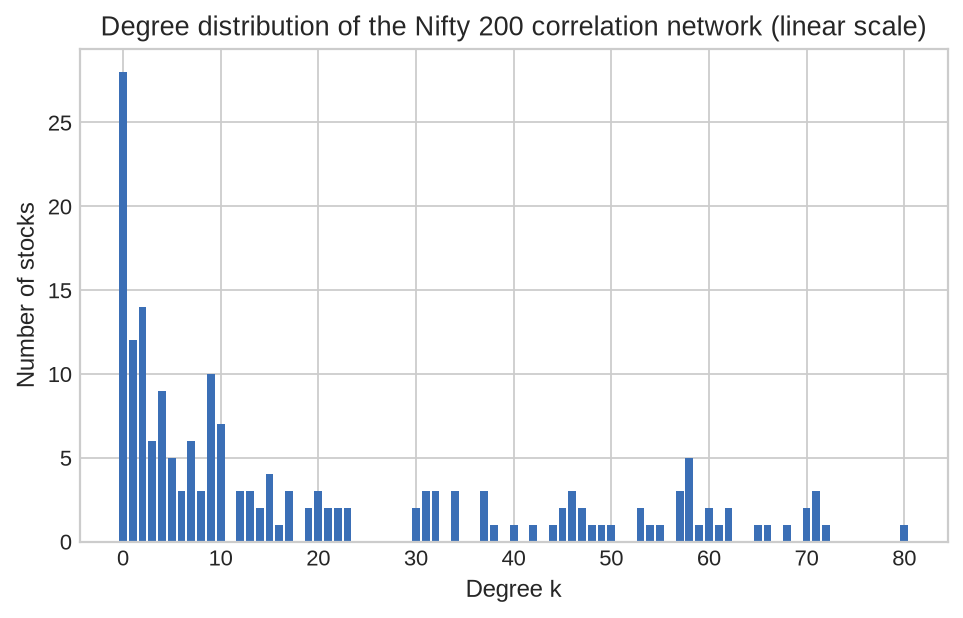
\includegraphics[width=\textwidth]{figures/degree_linear.png}
\caption{Linear scale.}
\label{fig:degree-linear}
\end{subfigure}\hfill
\begin{subfigure}[b]{0.48\textwidth}
\centering
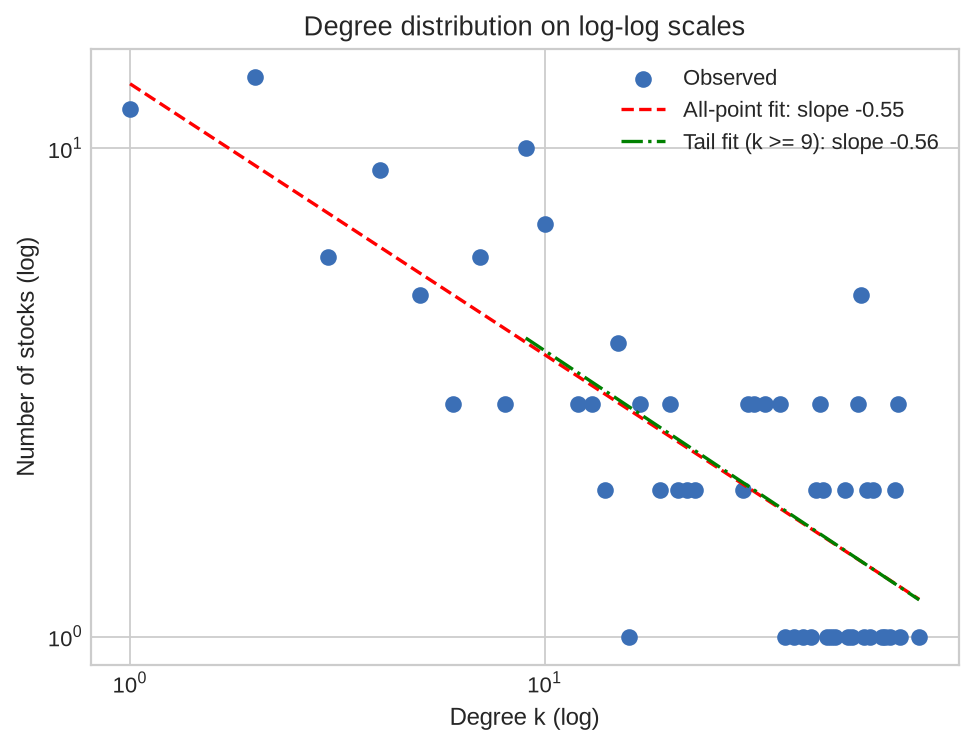
\includegraphics[width=\textwidth]{figures/degree_loglog.png}
\caption{Log--log scale, with least-squares fits over all points and over the tail.}
\label{fig:degree-loglog}
\end{subfigure}
\caption{Degree distribution of the Nifty 200 correlation network.}
\label{fig:degree}
\end{figure}

\begin{table}[!ht]
\centering
\caption{Summary of the degree distribution and log-log fits}
\label{tab:degree}
\begin{tabular}{ll}
\toprule
Statistic & Value \\
\midrule
Mean degree & 19.69 \\
Median degree & 9 \\
Maximum degree & 80 \\
Standard deviation & 22.37 \\
Isolated nodes & 28 \\
Log-log slope (all points) & -0.55 \\
R-squared (all points) & 0.60 \\
Log-log slope (tail) & -0.56 \\
R-squared (tail) & 0.33 \\
\bottomrule
\end{tabular}
\end{table}


% ---------------------------------------------------------------------------
% Code snippet: degree distribution and log-log least-squares fits
% Source file: src/03_analyses.py
% Suggested placement: Section 3.2 (Degree distribution).
% Uses the shared 'python' listings style defined in main.tex.
% ---------------------------------------------------------------------------
\begin{lstlisting}[style=python]
degrees = np.array([d for _, d in graph.degree()])
counts = np.bincount(degrees, minlength=degrees.max() + 1)
k = np.arange(len(counts))

# Ignore k = 0 (isolates) and empty bins on log axes
positive = k[(counts > 0) & (k > 0)]
freq = counts[(counts > 0) & (k > 0)]

# Fit over all points
slope, intercept, r_value, _, _ = stats.linregress(
    np.log(positive), np.log(freq))

# Fit over the tail, k >= max(5, median degree)
tail = positive >= max(5, int(np.median(degrees)))
tail_slope, tail_intercept, tail_r, _, _ = stats.linregress(
    np.log(positive[tail]), np.log(freq[tail]))

fig, ax = plt.subplots(figsize=(7, 5))
ax.scatter(positive, freq, s=42, label="Observed")
xs = np.logspace(np.log10(positive.min()),
                 np.log10(positive.max()), 100)
ax.plot(xs, np.exp(intercept) * xs ** slope, "r--",
        label=f"All-point fit: slope {slope:.2f}")
ax.set_xscale("log")
ax.set_yscale("log")
\end{lstlisting}


\subsection{Top-10 stocks according to centrality}
The three leaderboards are given in Tables~\ref{tab:top10-degree}--%
\ref{tab:top10-eigenvector}.
Degree and eigenvector centralities largely agree (Spearman
$\rho=0.94$, Table~\ref{tab:centrality-corr}). Degree is led by
\texttt{DLF.NS}, \texttt{RECLTD.NS}, \texttt{AMBUJACEM.NS},
\texttt{IRCTC.NS} and \texttt{TATAPOWER.NS}; the eigenvector leaderboard
contains the same names plus \texttt{CANBK.NS} in third place (with
\texttt{TATAPOWER.NS} sixth). Betweenness varies:
\texttt{INDHOTEL.NS}, \texttt{ETERNAL.NS}, \texttt{BIOCON.NS},
\texttt{NAUKRI.NS} and \texttt{LAURUSLABS.NS} act as bridges.

To quantify this agreement we use Spearman's rank correlation coefficient.
Instead of correlating the raw scores, Spearman correlates the \emph{ranks} of
the stocks, so it measures how monotonic the relationship is on a scale from
$-1$ to $+1$. This is appropriate here because the three centralities have very
different numerical ranges and skewed distributions --- for example, many
stocks outside the giant component have exactly zero eigenvector centrality ---
so a Pearson correlation would be dominated by a few large values. Spearman
instead answers the economically meaningful question of whether a stock that
ranks highly on one centrality also ranks highly on another. The value of
$0.94$ therefore confirms that degree and eigenvector centrality identify
essentially the same prominent stocks, while the much lower correlations
involving betweenness show that bridges form a distinct structural group.

\begin{table}[!ht]
\centering
\caption{Top-10 stocks by degree centrality}
\label{tab:top10-degree}
\begin{tabular}{llll}
\toprule
Rank & Company & Sector & Centrality \\
\midrule
1 & DLF Ltd. & Realty & 0.432 \\
2 & REC Ltd. & Financial Services & 0.389 \\
3 & Ambuja Cements Ltd. & Construction Materials & 0.384 \\
4 & Indian Railway Catering And Tourism Corporation Ltd. & Consumer Services & 0.384 \\
5 & Tata Power Co. Ltd. & Power & 0.384 \\
6 & Bharat Heavy Electricals Ltd. & Capital Goods & 0.378 \\
7 & Canara Bank & Financial Services & 0.378 \\
8 & Power Finance Corporation Ltd. & Financial Services & 0.368 \\
9 & GAIL (India) Ltd. & Oil Gas \& Consumable Fuels & 0.357 \\
10 & Bharat Electronics Ltd. & Capital Goods & 0.351 \\
\bottomrule
\end{tabular}
\end{table}

\begin{table}[!ht]
\centering
\caption{Top-10 stocks by betweenness centrality}
\label{tab:top10-betweenness}
\begin{tabular}{llll}
\toprule
Rank & Company & Sector & Centrality \\
\midrule
1 & Indian Hotels Co. Ltd. & Consumer Services & 0.100 \\
2 & Eternal Ltd. & Consumer Services & 0.089 \\
3 & Biocon Ltd. & Healthcare & 0.082 \\
4 & Info Edge (India) Ltd. & Consumer Services & 0.082 \\
5 & Laurus Labs Ltd. & Healthcare & 0.075 \\
6 & L\&T Finance Ltd. & Financial Services & 0.059 \\
7 & REC Ltd. & Financial Services & 0.047 \\
8 & DLF Ltd. & Realty & 0.042 \\
9 & Aditya Birla Capital Ltd. & Financial Services & 0.042 \\
10 & Bharat Heavy Electricals Ltd. & Capital Goods & 0.034 \\
\bottomrule
\end{tabular}
\end{table}

\begin{table}[!ht]
\centering
\caption{Top-10 stocks by eigenvector centrality (giant component)}
\label{tab:top10-eigenvector}
\begin{tabular}{llll}
\toprule
Rank & Company & Sector & Centrality \\
\midrule
1 & DLF Ltd. & Realty & 0.166 \\
2 & REC Ltd. & Financial Services & 0.165 \\
3 & Canara Bank & Financial Services & 0.163 \\
4 & Indian Railway Catering And Tourism Corporation Ltd. & Consumer Services & 0.162 \\
5 & Ambuja Cements Ltd. & Construction Materials & 0.162 \\
6 & Tata Power Co. Ltd. & Power & 0.162 \\
7 & Power Finance Corporation Ltd. & Financial Services & 0.162 \\
8 & Bharat Heavy Electricals Ltd. & Capital Goods & 0.160 \\
9 & GAIL (India) Ltd. & Oil Gas \& Consumable Fuels & 0.160 \\
10 & Punjab National Bank & Financial Services & 0.152 \\
\bottomrule
\end{tabular}
\end{table}

\begin{table}[!ht]
\centering
\caption{Spearman rank correlations between centrality measures}
\label{tab:centrality-corr}
\begin{tabular}{llll}
\toprule
Measure & Degree & Betweenness & Eigenvector \\
\midrule
Degree & 1.000 & 0.738 & 0.937 \\
Betweenness & 0.738 & 1.000 & 0.672 \\
Eigenvector & 0.937 & 0.672 & 1.000 \\
\bottomrule
\end{tabular}
\end{table}

\begin{table}[!ht]
\centering
\caption{Mean local clustering coefficient by sector, highest to lowest}
\label{tab:clustering-sector}
\begin{tabular}{lll}
\toprule
Sector & Stocks & Mean clustering \\
\midrule
Information Technology & 10 & 0.901 \\
Oil Gas \& Consumable Fuels & 9 & 0.828 \\
Power & 9 & 0.806 \\
Realty & 6 & 0.733 \\
Services & 4 & 0.708 \\
Construction & 2 & 0.688 \\
Metals \& Mining & 11 & 0.674 \\
Construction Materials & 3 & 0.612 \\
Financial Services & 45 & 0.604 \\
Automobile and Auto Components & 13 & 0.579 \\
Chemicals & 5 & 0.552 \\
Fast Moving Consumer Goods & 14 & 0.541 \\
Capital Goods & 20 & 0.520 \\
Telecommunication & 4 & 0.436 \\
Healthcare & 15 & 0.248 \\
Consumer Durables & 7 & 0.245 \\
Consumer Services & 8 & 0.238 \\
Textiles & 1 & 0.000 \\
\bottomrule
\end{tabular}
\end{table}


\subsection{Local clustering and sector homophily}
The average clustering coefficient is $0.570$, more than five times the value
$0.106$ for an Erd\H{o}s--R\'enyi graph with the same size and density. Of the 1831
edges, 503 ($27.5\%$) join stocks in the same NSE industry, versus a baseline
of $10.0\%$: a homophily ratio of $2.75$, with modularity $0.122$. Sectors with
the tightest triangles are Information Technology (mean local clustering
$0.901$), Oil \& Gas ($0.828$) and Power ($0.806$); Healthcare ($0.248$) and
Consumer Services ($0.238$) are much looser
(Table~\ref{tab:clustering-sector}). Means for sectors with fewer than five
stocks are based on very few observations; Textiles, with a single stock, is
zero by construction. The distribution of local clustering is
shown in Figure~\ref{fig:clustering}; Figure~\ref{fig:network} shows a
sector-level aggregation and the giant component. At the sector level,
Financial Services is the dominant hub, whereas IT is almost self-contained:
40 of its 43 edges stay inside the sector.

% ---------------------------------------------------------------------------
% Code snippet: clustering, Erdos-Renyi baseline, sector homophily, modularity
% Source file: src/03_analyses.py
% Suggested placement: Section 3.4 (Local clustering and sector homophily).
% Uses the shared 'python' listings style defined in main.tex.
% ---------------------------------------------------------------------------
\begin{lstlisting}[style=python]
local = nx.clustering(graph)
avg = nx.average_clustering(graph)
random_avg = nx.average_clustering(nx.gnp_random_graph(
    graph.number_of_nodes(), nx.density(graph),
    seed=config.RANDOM_SEED))

sector = {n: graph.nodes[n]["sector"] for n in graph.nodes()}
sector_counts = pd.Series(list(sector.values())).value_counts()
same = sum(1 for u, v in graph.edges() if sector[u] == sector[v])

# Baseline fraction expected for random edges among these sector sizes
n = graph.number_of_nodes()
baseline = sum(s * (s - 1) for s in sector_counts) / (n * (n - 1))

# Modularity of the partition induced by NSE industry labels
communities = [
    [node for node in graph.nodes()
     if graph.nodes[node]["sector"] == s]
    for s in sector_counts.index
]
modularity = nx.community.modularity(graph, communities)

summary = {
    "average_clustering": avg,
    "random_graph_clustering": random_avg,
    "observed_same_sector_fraction": same / graph.number_of_edges(),
    "baseline_same_sector_fraction": baseline,
    "homophily_ratio": (same / graph.number_of_edges()) / baseline,
    "sector_modularity": modularity,
}
\end{lstlisting}


\begin{figure}[htbp]
\centering
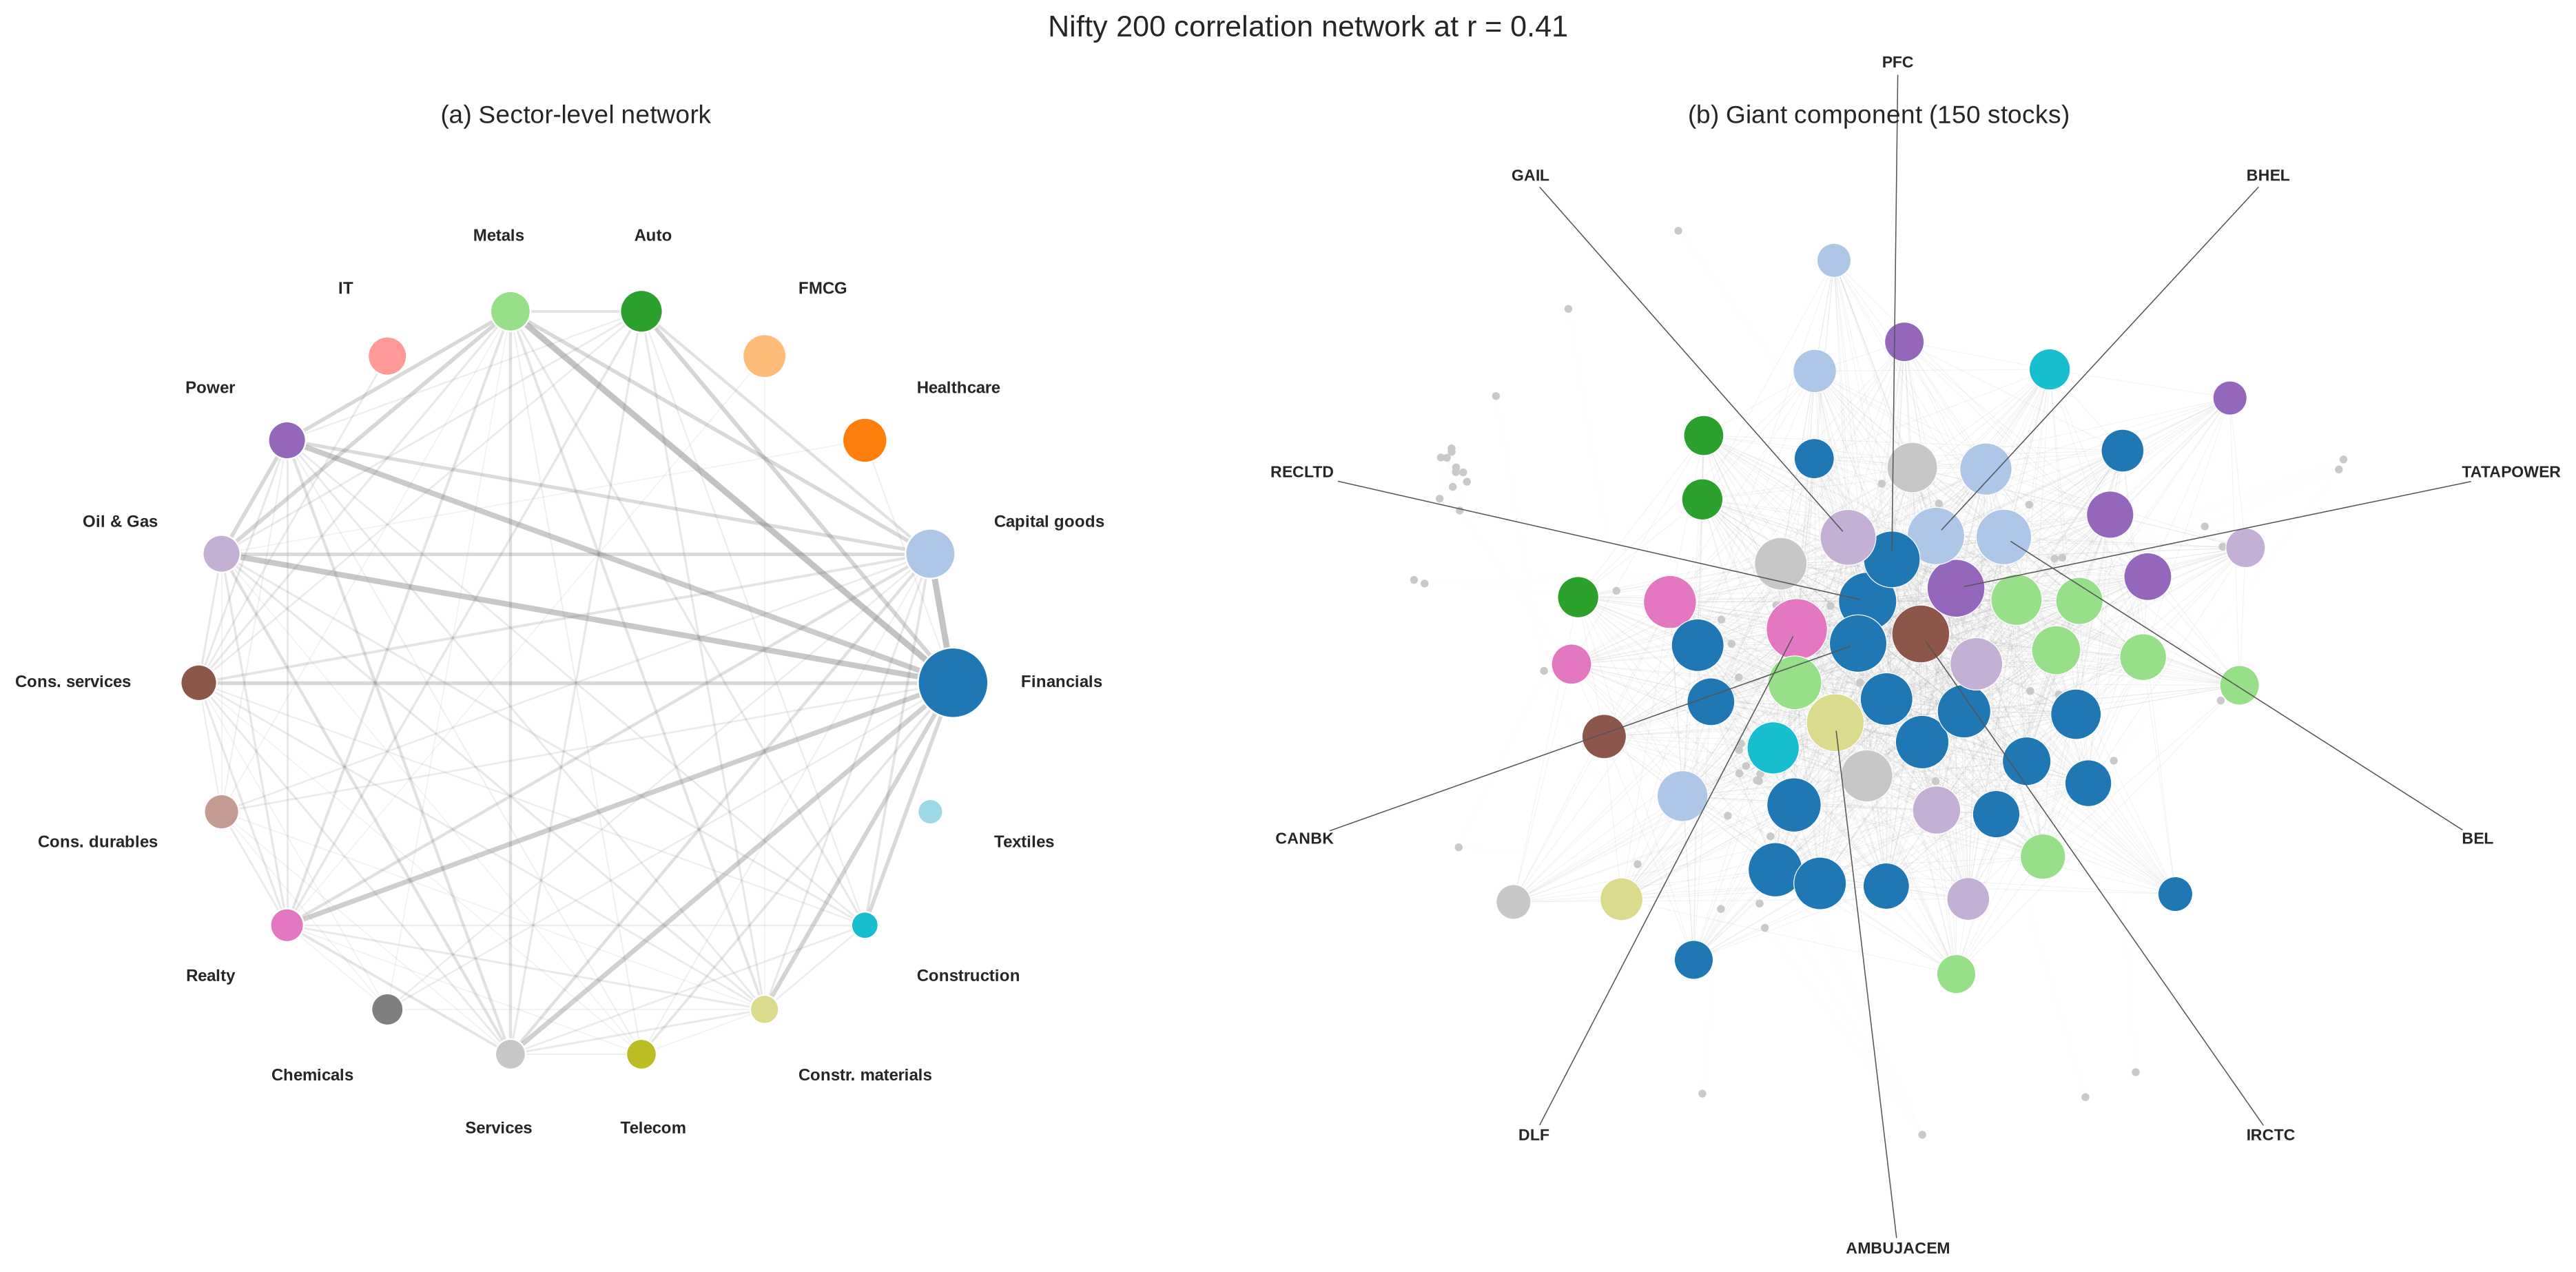
\includegraphics[width=\textwidth]{figures/network_sectors.png}
\caption{Primary correlation network at $r=0.41$. (a)~Sector-level
aggregation: nodes are NSE industries, sized by the number of stocks, and
edges are weighted by the number of cross-sector correlations. (b)~Giant
component (150 stocks): the 60 highest-degree stocks are coloured (node size
increasing with degree) and the ten largest hubs are labelled; the remaining
stocks are small grey dots. Isolated stocks are omitted.}
\label{fig:network}
\end{figure}

% Optional: spring-layout drawing code for this figure
% % ---------------------------------------------------------------------------
% Code snippet: force-directed sector-coloured network visualisation
% Source file: src/03_analyses.py
% Suggested placement: Figure 5 (sector-coloured network) or Section 2.4.
% Uses the shared 'python' listings style defined in main.tex.
% ---------------------------------------------------------------------------
\begin{lstlisting}[style=python]
# Force-directed layout: fixed seed keeps the figure reproducible
pos = nx.spring_layout(graph, seed=config.RANDOM_SEED,
                       k=0.12, iterations=120)

colour_map = mpl.colormaps["tab20"]
colours = {s: colour_map(i / max(len(sector_list) - 1, 1))
           for i, s in enumerate(sector_list)}
node_sizes = {n: 12 + 2.0 * degree for n, degree in graph.degree()}

nx.draw_networkx_edges(graph, pos, alpha=0.12, width=0.4,
                       edge_color="#666666")
for sector in sector_list:
    nodes = [n for n in graph.nodes()
             if graph.nodes[n]["sector"] == sector]
    nx.draw_networkx_nodes(
        graph, pos, nodelist=nodes,
        node_size=[node_sizes[n] for n in nodes],
        node_color=[colours[sector]], label=sector,
        edgecolors="white", linewidths=0.3,
    )
\end{lstlisting}


\begin{figure}[H]
\centering
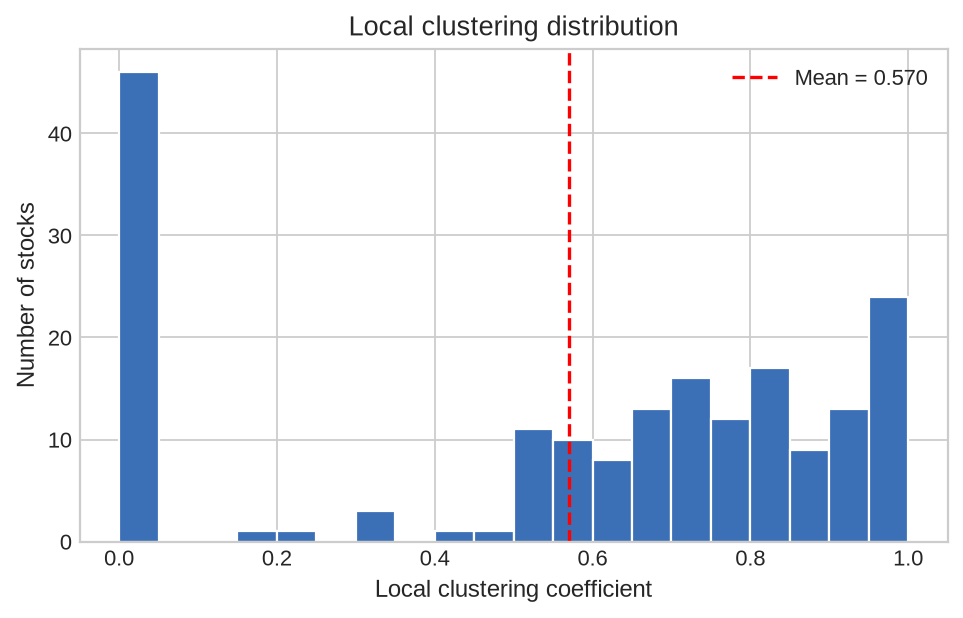
\includegraphics[width=0.85\textwidth]{figures/clustering_distribution.png}
\caption{Distribution of local clustering coefficients.}
\label{fig:clustering}
\end{figure}



\subsection{Threshold sensitivity}
Figure~\ref{fig:sensitivity} and Table~\ref{tab:sensitivity} show the ``what-if''
study. Raising $r$ from 0.30 to 0.75 reduces the number of edges from 5684 to
12 and the giant component from $98.9\%$ to $1.6\%$ of the stocks. The average
path length on the giant component first \emph{increases} (1.86 at $r=0.30$ to
2.79 at $r=0.40$) as the graph becomes sparser, then becomes erratic once the
giant component fragments (2.12 at 0.45, 3.12 at 0.55). The decisive
connectivity loss occurs between $r=0.40$ and $r=0.50$, where the giant
component falls from $82.8\%$ to $45.7\%$ of the network.

% ---------------------------------------------------------------------------
% Code snippet: threshold sensitivity sweep
% Source file: src/03_analyses.py
% Suggested placement: Section 3.5 (Threshold sensitivity).
% Uses the shared 'python' listings style defined in main.tex.
% ---------------------------------------------------------------------------
\begin{lstlisting}[style=python]
values = corr.to_numpy()
rows = []
for r in config.SWEEP_THRESHOLDS:              # 0.30 ... 0.75
    graph = nx.from_numpy_array(adjacency(values, r))
    metrics = graph_metrics(graph)

    # Average shortest path length on the giant component only
    largest = max(nx.connected_components(graph), key=len)
    subgraph = graph.subgraph(largest)
    path = (nx.average_shortest_path_length(subgraph)
            if subgraph.number_of_nodes() > 1 else np.nan)

    rows.append({"threshold": r, **metrics,
                 "avg_path_length_giant": path})

sweep = pd.DataFrame(rows)
sweep.to_csv(config.RESULTS_DIR / "threshold_sensitivity.csv", index=False)
\end{lstlisting}


\begin{figure}[htbp]
\centering
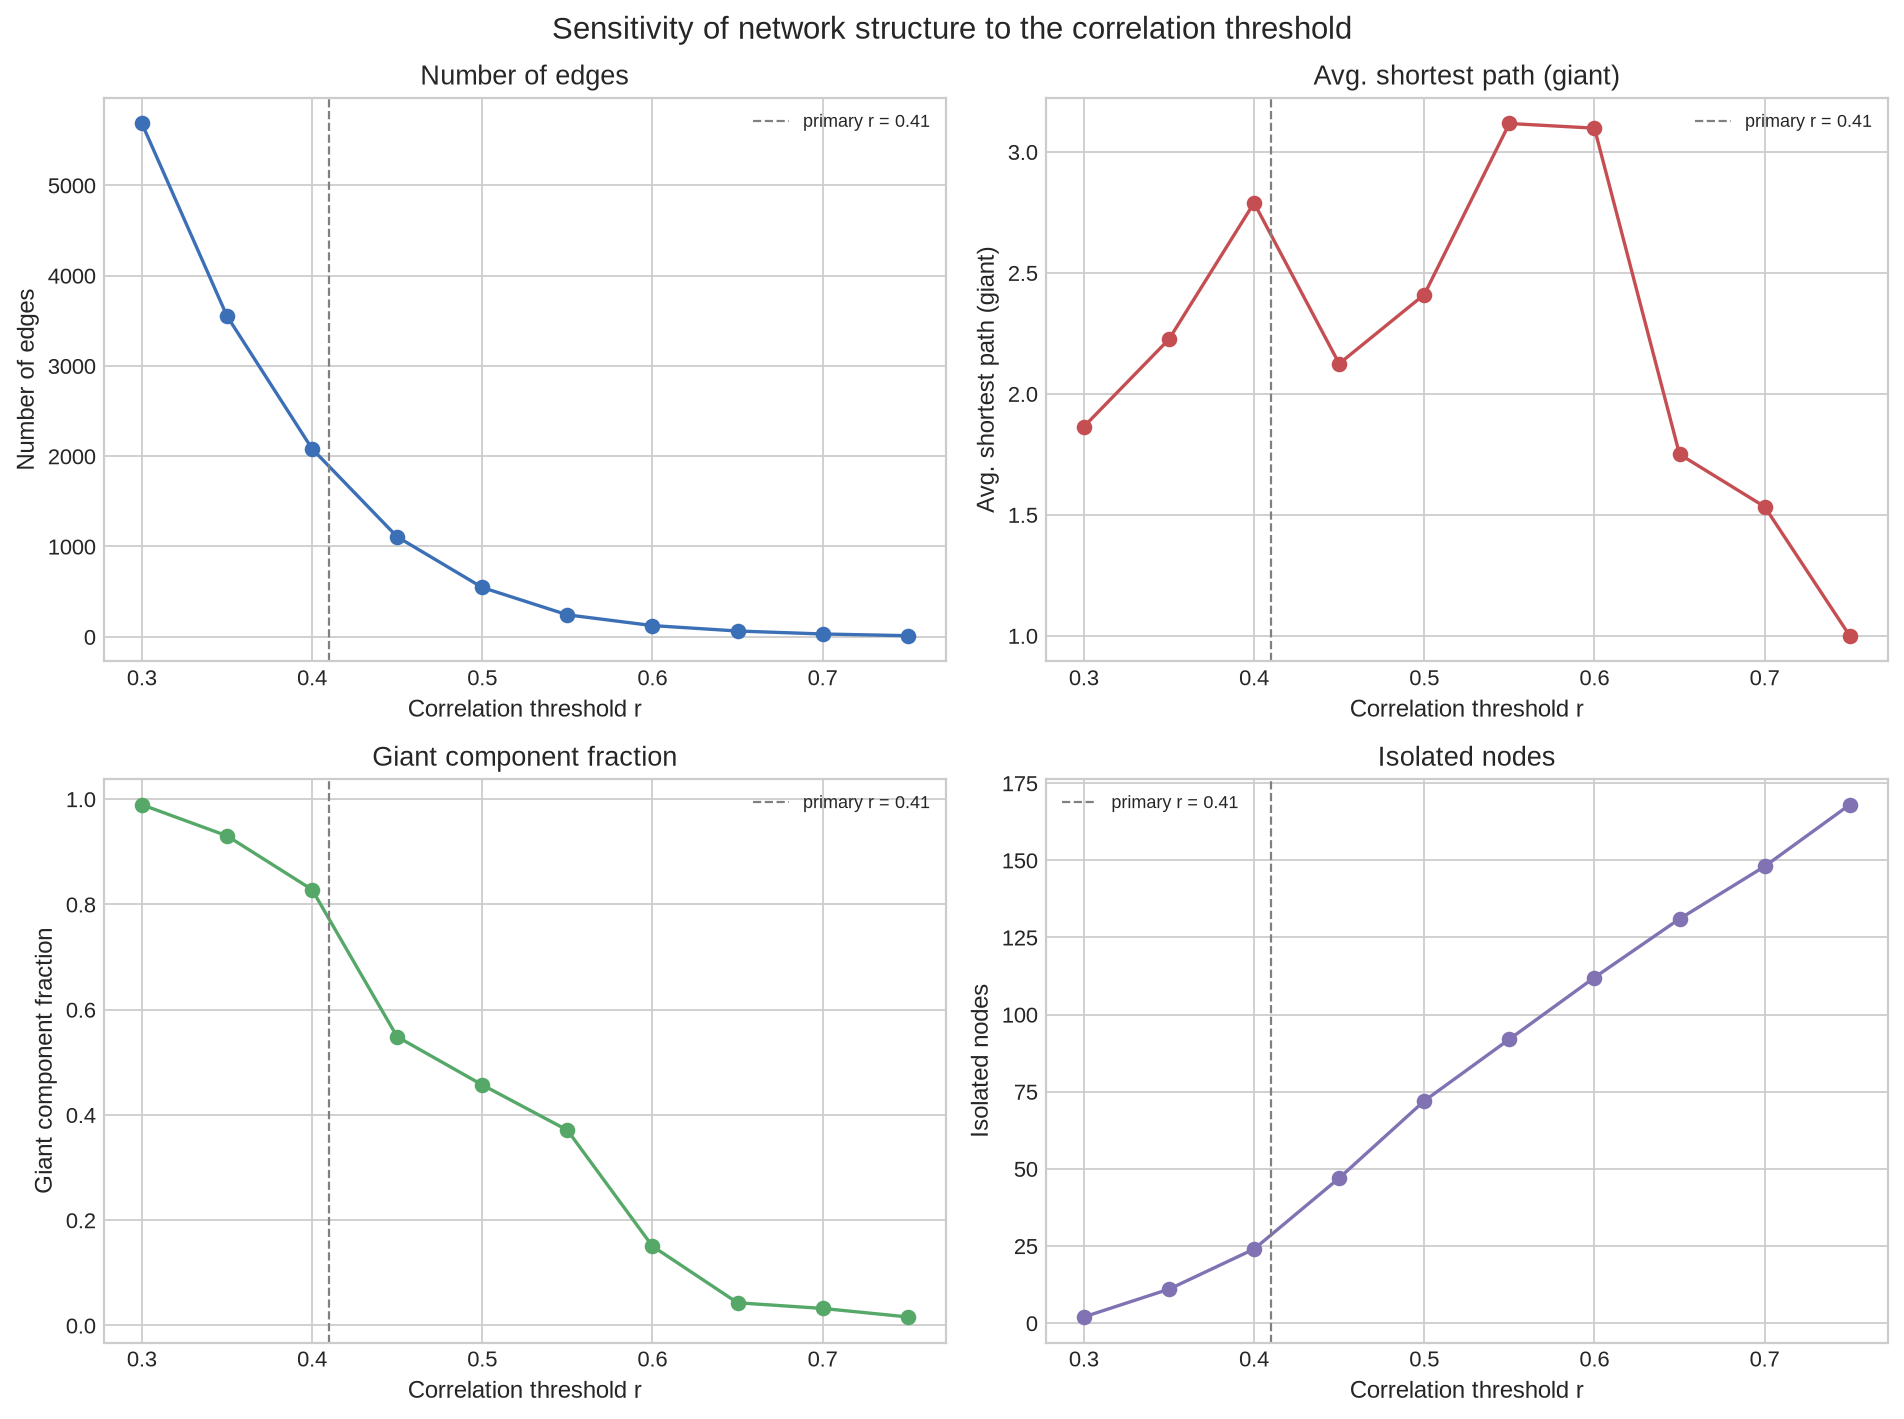
\includegraphics[width=\textwidth]{figures/threshold_sensitivity.png}
\caption{Edge count, average shortest path length on the giant component,
giant-component fraction and number of isolated nodes as the correlation
threshold varies. The dashed line marks the primary threshold $r=0.41$.}
\label{fig:sensitivity}
\end{figure}

\begin{table}[!ht]
\centering
\caption{Sensitivity of network metrics to the correlation threshold}
\label{tab:sensitivity}
\begin{tabular}{lllll}
\toprule
$r$ & Edges & Path length & Giant fraction & Isolates \\
\midrule
0.300 & 5684 & 1.864 & 0.989 & 2 \\
0.350 & 3552 & 2.225 & 0.930 & 11 \\
0.400 & 2082 & 2.789 & 0.828 & 24 \\
0.450 & 1107 & 2.124 & 0.548 & 47 \\
0.500 & 546 & 2.410 & 0.457 & 72 \\
0.550 & 243 & 3.117 & 0.371 & 92 \\
0.600 & 124 & 3.098 & 0.151 & 112 \\
0.650 & 64 & 1.750 & 0.043 & 131 \\
0.700 & 31 & 1.533 & 0.032 & 148 \\
0.750 & 12 & 1.000 & 0.016 & 168 \\
\bottomrule
\end{tabular}
\end{table}


\section{Interpretation and discussion}
\label{sec:discussion}

\paragraph{Hubs versus index heavyweights.}
The network's most connected stocks are not the familiar Nifty heavyweights.
At $r=0.41$, Reliance ranks 69th in degree, TCS 102nd and HDFC Bank 82nd;
TCS and Infosys have eigenvector scores of only $1.5\times10^{-7}$ and
$1.1\times10^{-6}$ respectively: effectively zero, but not because they lie
outside the giant component --- both are members of it. Their co-movement
partners are mostly other information-technology stocks with similarly tiny
eigenvector scores, so eigenvector centrality assigns them almost no weight.
This does not mean these companies are unimportant: their returns are dominated
by idiosyncratic or index-level moves rather than strong
pairwise co-movement with many other constituents. Instead, the hubs are
real-estate, public-sector finance, infrastructure and power stocks
(\texttt{DLF}, \texttt{REC}, \texttt{PFC}, \texttt{CANBK}, \texttt{TATAPOWER}). One possible explanation is that these companies share exposure to common macroeconomic factors, including interest-rate expectations, credit conditions and infrastructure-related policy developments.

\paragraph{Bridges.}
Betweenness centrality highlights a different set: Indian Hotels, Eternal
(Zomato), Biocon, Info Edge and Laurus Labs. These consumer-services and
healthcare names bridge otherwise separate sector blocks; financial-services
bridges (L\&T Finance, REC and Aditya Birla Capital) appear just below them in
ranks 6--10. They do not score as highly on degree and eigenvector
centrality, illustrating why the three measures capture different
structural roles.

\paragraph{Sector homophily and triangles.}
High clustering well above the random-graph baseline and a homophily ratio of
$2.75$ confirm that correlation triangles form within industries. IT, oil/gas
and power stocks share strong common factors (global technology cycles, crude
prices, regulated tariffs), producing tight cliques. Healthcare and consumer
services are more heterogeneous, so their stocks bridge sectors rather than
forming cliques. The moderate modularity ($0.122$) indicates sector structure
is visible but far from a clean partition --- many cross-sector links remain,
as expected in an integrated market.

\paragraph{Robustness.}
The sharp transition around $r=0.40$--$0.50$ is the percolation-like behaviour
expected from thresholding a dense correlation matrix: connectivity is robust
to modest tightening but collapses quickly beyond a critical threshold.

\section{Conclusion}
\label{sec:conclusion}
This assignment was a wonderful exercise to implement the concepts learned during class to a real-world dataset. The idea of modelling the stock market as a graph with edges defined this way was nice.

We built a 186-node, 1831-edge network of Nifty~200 stocks from three years of
daily log returns and a correlation threshold of $0.41$. The degree
distribution is right-skewed with a weak heavy tail but is not cleanly
scale-free. Degree and eigenvector centrality identify public-sector finance,
real-estate and infrastructure hubs, while betweenness identifies consumer and
healthcare bridges.
Clustering is more than five times the random baseline and same-sector edges
are $2.75$ times more common than chance, confirming sector homophily. The
connectivity sweep shows a rapid loss of the giant component between $r=0.40$
and $r=0.50$. Overall, simple correlation thresholding already reveals
economically meaningful structure: centrality, clustering and sector
homophily point to the same set of hubs and bridges.

\end{document}

